\section{Introducing Contexts}
\label{tut_contexts}
\index{context}

\tick{\textbf{Goals:} In this section we introduce contexts that apply to the theoretical concepts that were introduced in the previous section (\ref{tut_mathematical_notation}). We will create a very simple model consisting of just one context file.
}

In this tutorial, we will create a model of the well known Agatha puzzle. Here is a brief description of the puzzle:

\textit{Someone in Dreadsbury Mansion killed Aunt Agatha. Agatha, the butler, and Charles live in Dreadsbury Mansion and are the only ones to live there. A killer always hates, and is no richer than his victim. Charles hates no one that Agatha hates. Agatha hates everybody except the butler. The butler hates everyone not richer than Aunt Agatha. The butler hates everyone whom Agatha hates. No one hates everyone. Who killed Agatha?}

Contexts are used to model static properties of a model, things that do not change over time. Whereas with machines we model the dynamic properties like the traffic light above.
The objective of this Section is to get familiar with contexts by modeling the Agatha puzzle.

\subsection{Create a Context}
\label{tut_create_context}
\index{context!creation of}

Create a new Event-B Project \textsf{File $\rangle$ New $\rangle$ Event-B Project}. Give the project the name \texttt{tutorial-05}. 

Next, create a new Event-B Component. Unlike in Section (\ref{tut_first_machine}) use \texttt{agatha} as the component name and mark the \textsf{Context} (\ref{context}) option in order to create a Context file instead of a Machine (\ref{machine}) file.

%\begin{figure}[!h]
%\begin{center}
%	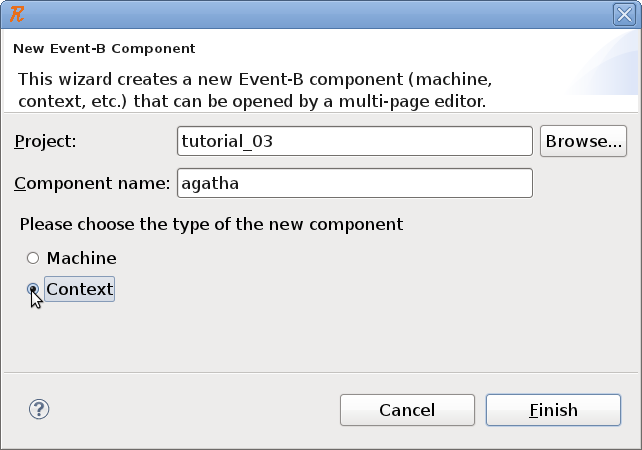
\includegraphics{img/tutorial/tut_05_agatha1.png}
%	\caption{New Event-B Component Wizard}
%	\label{fig_tut_05_new_component}
%\end{center}
%\end{figure}

Click on \textsf{Finish}. Rodin should start the editor with the created Context file (see Figure \ref{fig_tut_05_context_file}).

\begin{figure}[!h]
\begin{center}
	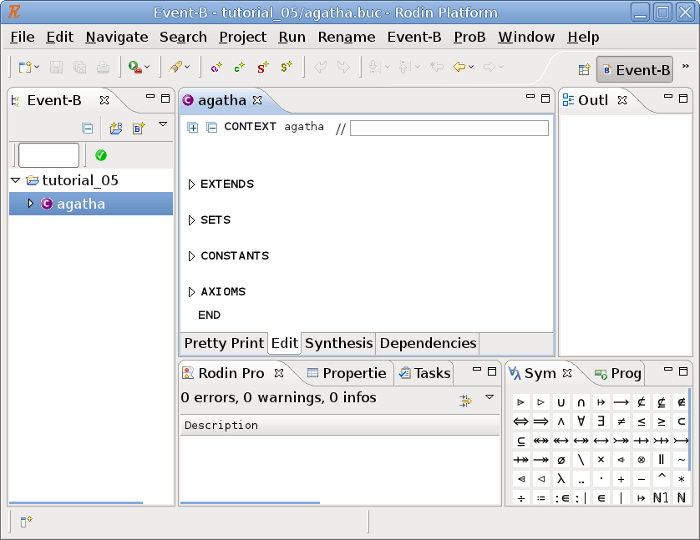
\includegraphics{img/tutorial/tut_05_agatha2.png}
	\caption{Context file opened with Structural Editor}
	\label{fig_tut_05_context_file}
\end{center}
\end{figure}

\subsection{Populate the Context}
\label{tut_populate_context}

In this section we model the Agatha puzzle step by step.

\subsubsection{Modelling the Persons}
\label{tut_modelling_persons}

We have three persons in the Agatha puzzle: Agatha herself, the butler and Charles. We model the three persons as constants (one constant for each person) in the corresponding \textsf{CONSTANTS} section:

\pencil{
\begin{description}
\CONSTANTS
	\begin{description}
		\Item{ Agatha }
		\Item{ butler }
		\Item{ Charles }
	\end{description}
\end{description}
}

These constants or persons respectively are part of a set:

\pencil{
\begin{description}
\SETS
	\begin{description}
		\Item{ persons }
	\end{description}
\end{description}
}

Now, the constants itself are not very useful since they have no type (In addition, the constants will be highlighted in red, indicating a problem). The semantics of the sets (\ref{sets}) and constants (\ref{constants_and_axioms}) are specified in the axioms (\ref{constants_and_axioms}). As already mentioned above the persons are part of the set \texttt{persons}. We model this by creating a partition (\ref{partition}) in the \textsf{AXIOMS} section: 

\pencil{
\begin{description}
\AXIOMS
	\begin{description}
		\nItemX{ person\_partition }{ partition(persons, \{ Agatha\} , \{ butler\} , \{ Charles\} ) }
	\end{description}
\end{description}
}

\warning{Please note the curly braces \{\} around the constants.  It's very easy to forget these, which will result in typing errors that are very hard to interpret for a novice.
}

\index{wizard!New Enumerated Set Wizard}
\info{The \textsf{New Enumerated Set Wizard} (\ref{enumerated_set_wizard}) allows you to create the constants, the set and the axiom automatically at the same time. To access this wizard, click on the \textsf{New Enumerated Set Wizard} tool bar item or find it under \textsf{ Event-B $\rangle$ New Enumerated Set Wizard}. This will bring up the wizard where we can enter the name of the set and the constants in the corresponding text fields. The wizard will create the enumarted set, the constants and the axiom automatically.}

\subsubsection{Modelling the Relations ``Persons who hate each other'' and ``Who's how rich''}

We create two more constants \texttt{hates} and \texttt{richer} to model the relations ``Persons who hate each other'' and ``Who's how rich''. The relations are abstract, which means that they say nothing about the concrete persons (Agatha, the butler and Charles). We define the concrete relationships between the persons later in this section.

The first constant \texttt{hates} is an arbitrary relation (\ref{relations}) between \texttt{persons}: 

\pencil{
\begin{description}
\AXIOMS
	\begin{description}
		\nItemX{ hate\_relation }{ hates \in  persons \rel  persons }
	\end{description}
\end{description}
}

The second constant \texttt{richer} is also a relation between \texttt{persons}:

\pencil{
\begin{description}
\AXIOMS
	\begin{description}
		\nItemX{ richer\_relation1 }{ richer \in  persons \rel  persons }
	\end{description}
\end{description}
}

However, we know that the relation is irreflexive (no person is richer than itself):

\pencil{
\begin{description}
\AXIOMS
	\begin{description}
		\nItemX{ richer\_relation2 }{ richer \binter  id = \emptyset }
	\end{description}
\end{description}
}

In addition, we know that the relation is transitive:

\pencil{
\begin{description}
\AXIOMS
	\begin{description}
		\nItemX{ richer\_relation3 }{ (\forall  x,y,z \qdot  ( x\mapsto y\in richer \land  y\mapsto z\in richer) \limp  x\mapsto z\in richer) }
	\end{description}
\end{description}
}

Finally, the relation is trichotomous (one person is always richer than the other or vice versa, never both directions):

\pencil{
\begin{description}
\AXIOMS
	\begin{description}
		\nItemX{ richer\_relation4 }{ (\forall  x,y \qdot x\in persons \land  y\in persons \land  x\neq y \limp  (x\mapsto y\in richer \leqv  y\mapsto  x \notin  richer)) }
	\end{description}
\end{description}
}

\subsubsection{Modelling the ``Crime''}

Since the objective of the puzzle is to find the killer, we have to create a new constant \texttt{killer} which is an element of \texttt{persons}:

\pencil{
\begin{description}
\CONSTANTS
	\begin{description}
		\Item{ killer }
	\end{description}
\AXIOMS
	\begin{description}
		\nItemX{ killer\_type }{ killer \in  persons }
	\end{description}
\end{description}
}

In addition, the puzzle have some more relationships between the different persons which are all modelled as axioms. We know that the killer hates his victim and is no richer than his victim:

\pencil{
\begin{description}
\AXIOMS
	\begin{description}
		\nItemX{ killer\_hates }{ killer \mapsto  Agatha \in  hates }
		\nItemX{ killer\_not\_richer }{ killer \mapsto  Agatha \notin  richer }
	\end{description}
\end{description}
}

Charles hates no one that Agatha hates and Agatha hates everybody except the butler:

\pencil{
\begin{description}
\AXIOMS
	\begin{description}
		\nItemX{ charles\_hates }{ hates[\{ Agatha\} ] \binter  hates[\{ Charles\} ] = \emptyset  }
		\nItemX{ agatha\_hates }{ hates[\{ Agatha\} ] = persons \setminus  \{ butler\}  }
	\end{description}
\end{description}
}

The butler hates everyone not richer than aunt Agatha and the butler hates everyone whom Agatha hates. However, no one hates everyone:

\pencil{
\begin{description}
\AXIOMS
	\begin{description}
		\nItemX{ butler\_hates\_1 }{ \forall x\qdot ( x\mapsto Agatha \notin  richer \limp  butler\mapsto x \in  hates) }
		\nItemX{ butler\_hates\_2 }{ hates[\{ Agatha\} ] \subseteq  hates[\{ butler\} ] \land 
		\\\hspace*{3,2 cm}  (\forall  x\qdot  x\in persons \limp  hates[\{ x\} ] \neq  persons) }
		\nItemX{ noone\_hates\_everyone }{ \forall  x \qdot  x \in  persons \land  hates[\{ x\} ] \neq  persons }
	\end{description}
\end{description}
}

Finally, we have to model the solution:

\pencil{
\begin{description}
\AXIOMS
	\begin{description}
		\nItemX{ solution }{ killer = Agatha }
	\end{description}
\end{description}
}

We mark the axiom \texttt{solution} as a theorem (\ref{theorem}) by clicking on the \textsf{not theorem} button as shown in figure \ref{fig_tut_05_mark_theorem}.

\begin{figure}[!h]
\begin{center}
	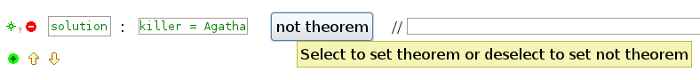
\includegraphics{img/tutorial/tut_05_agatha3.png}
	\caption{Mark an Axiom as Theorem}
	\label{fig_tut_05_mark_theorem}
\end{center}
\end{figure}

\info{Theorems describe properties that are expected to be able to be derived from the axioms.}

\index{ProB}
\begin{rodin-plugin}{img/prob.png}{ProB}%
  You can use ProB to animate contexts, too.
  Just right-click on the context in the explorer and select \textsf{Start Animation / Model Checking}.
  If ProB finds solutions for the specified constants that fulfil the axioms,
  an event ``\texttt{SETUP\_CONTEXT}'' is enabled that assigns values to the constants.

  In our example, ProB should find a solution where Agatha is the murder. You can actually inspect
  the axioms and the theorem in the state view to see why they are fulfilled.
\end{rodin-plugin}

This concludes the tutorial. The following section shows the complete Context.

\subsection{The Final Context} 
\label{tut_final_context}

\begin{description}
\CONTEXT{agatha}
\SETS
	\begin{description}
		\Item{ persons }
	\end{description}
\CONSTANTS
	\begin{description}
		\Item{ Agatha }
		\Item{ butler }
		\Item{ Charles }
		\Item{ hates }
		\Item{ richer }
		\Item{ killer }
	\end{description}
\AXIOMS
	\begin{description}
		\nItemX{ person\_partition }{ partition(persons, \{ Agatha\} , \{ butler\} , \{ Charles\} ) }
		\nItemX{ hate\_relation }{ hates \in  persons \rel  persons }
		\nItemX{ richer\_relation }{ richer \in  persons \rel  persons \land 
		\\\hspace*{3,4 cm}  richer \binter  id = \emptyset  \land 
		\\\hspace*{3,4 cm}  (\forall  x,y,z \qdot  ( x\mapsto y\in richer \land  y\mapsto z\in richer) \limp  x\mapsto z\in richer) \land 
		\\\hspace*{3,4 cm}  (\forall  x,y \qdot x\in persons \land  y\in persons \land  x\neq y \limp  (x\mapsto y\in richer \leqv  y\mapsto x \notin  richer)) }
		\nItemX{ killer\_type }{ killer \in  persons }
		\nItemX{ killer\_hates }{ killer \mapsto  Agatha \in  hates }
		\nItemX{ killer\_not\_richer }{ killer \mapsto  Agatha \notin  richer }
		\nItemX{ charles\_hates }{ hates[\{ Agatha\} ] \binter  hates[\{ Charles\} ] = \emptyset  }
		\nItemX{ agatha\_hates }{ hates[\{ Agatha\} ] = persons \setminus  \{ butler\}  }
		\nItemX{ butler\_hates\_1 }{ \forall x\qdot ( x\mapsto Agatha \notin  richer \limp  butler\mapsto x \in  hates) }
		\nItemX{ butler\_hates\_2 }{ hates[\{ Agatha\} ] \subseteq  hates[\{ butler\} ] \land 
		\\\hspace*{3,2 cm}  (\forall  x\qdot  x\in persons \limp  hates[\{ x\} ] \neq  persons) }
		\nItemX{ noone\_hates\_everyone }{ \forall  x \qdot  x \in  persons \land  hates[\{ x\} ] \neq  persons }
		\nItemX{ solution }  { \fbox{theorem} ~ killer = Agatha }
	\end{description}
\END
\end{description}


%%% Local Variables: 
%%% mode: latex
%%% TeX-master: "rodin-doc"
%%% End: 
